\documentclass{article}
\usepackage[utf8]{inputenc}
\usepackage[dutch]{varioref}
\usepackage[autostyle]{csquotes} 
\usepackage[dutch]{babel}
\usepackage{listings}
\usepackage{pdfpages}
\usepackage{url}
\usepackage{natbib}
\usepackage{graphicx}

\title{Stageverslag}
\author{\mbox{Pieter-Jan} Robrecht}
\date{Maart 2016}

\begin{document}

%\maketitle
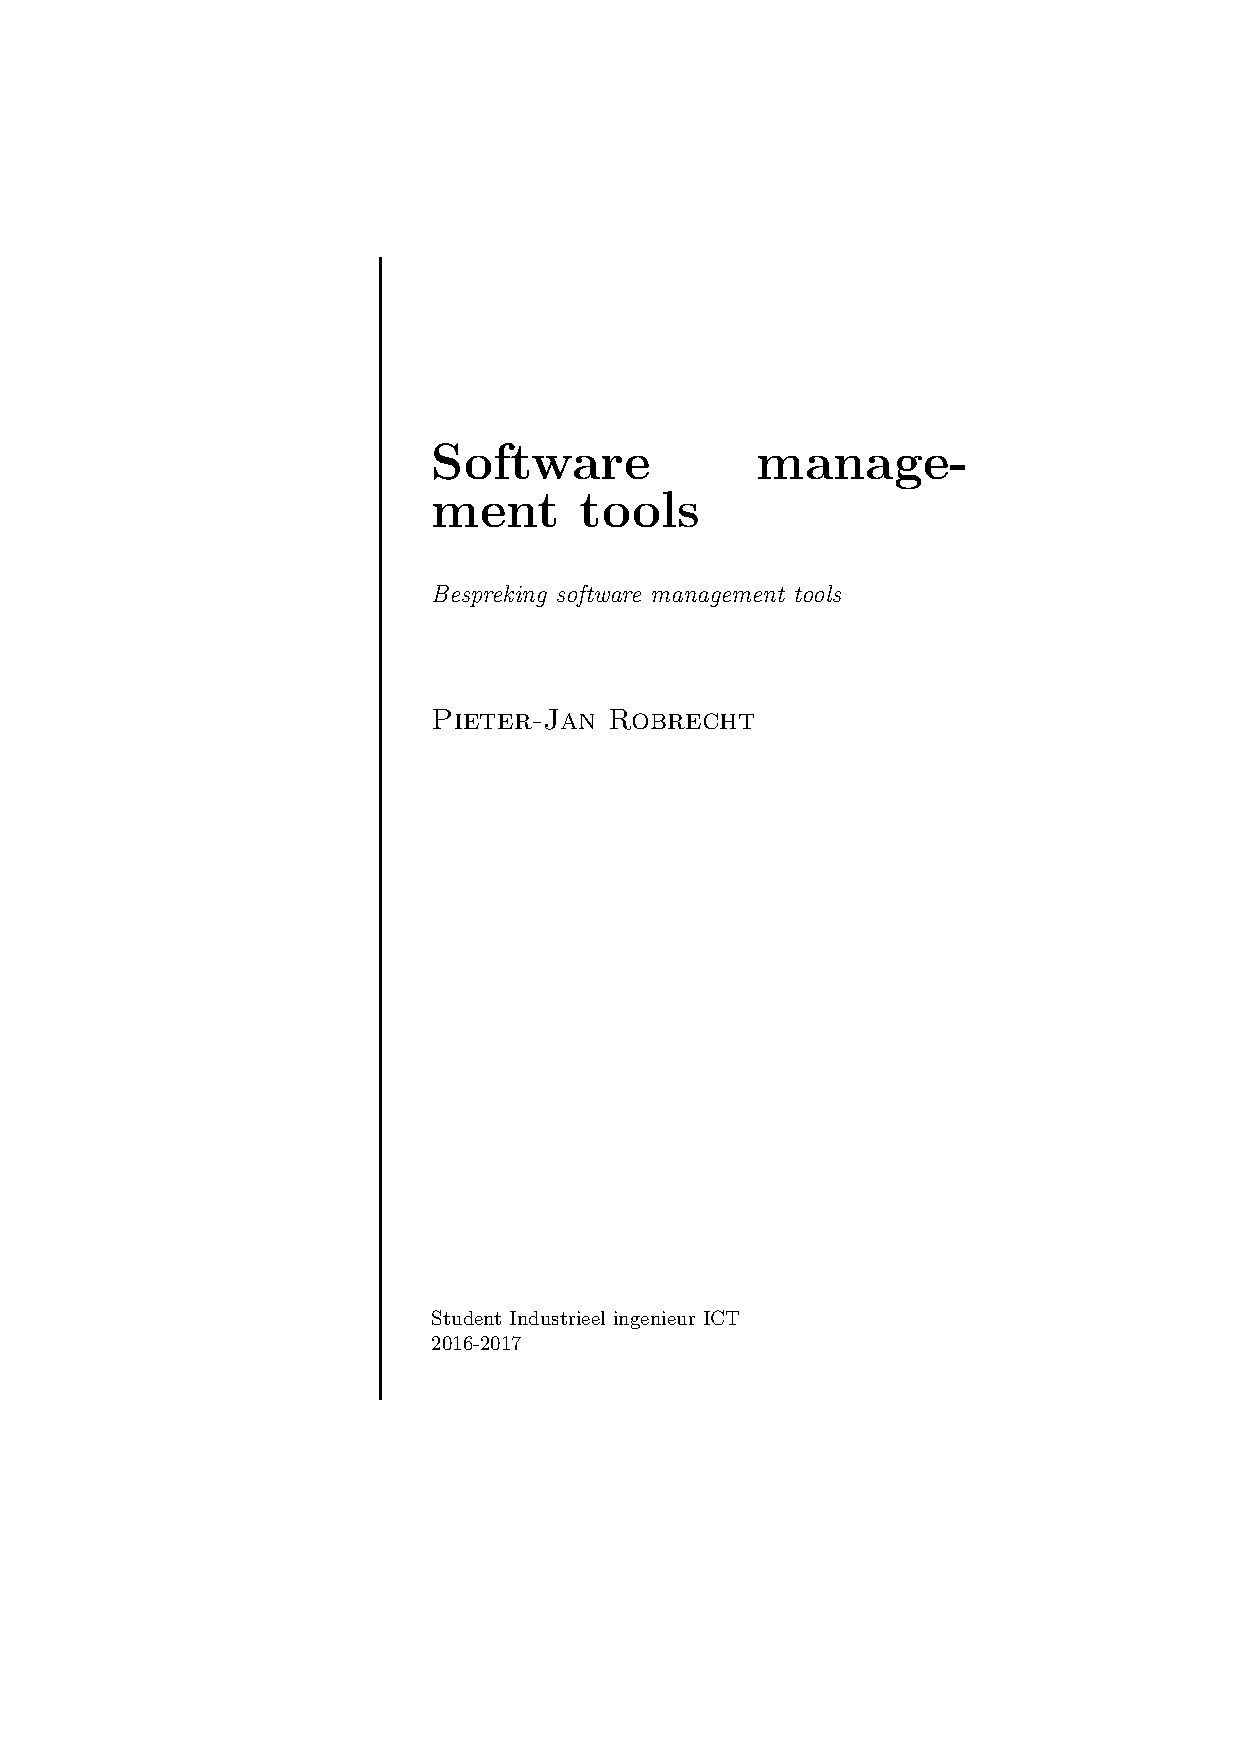
\includepdf{titel/management.pdf}

%Volgende lijn is om de titelpagina geen paginanummer te geven
\clearpage
\setcounter{page}{1}

\tableofcontents
\lstlistoflistings
\clearpage

\section{Inleiding}
Hieronder bespreek ik enkele tools die gebruikt zouden kunnen worden voor het maken van het software management platform.\citep{thread309256}
Voor dit te verwezenlijken zou er gebruik kunnen maakt worden van een simpel log bestand waarin alle ok/nok komen die de testtoren terugsturen.
Het zou mooi zijn, mocht ik gebruik kunnen maken van een tool waarmee ik een goede GUI heb waarin alles zichtbaar is.

\section{Bespreking}
\subsection{ElectricFlow \citep{electricMain}}
Een eerste tool die ik kort zal toelichten is Electric Flow.
Deze tool bezit geen uitgebreide documentatie en ik moet dus van de hoofdpagina uitgaan.
Een voordeel van deze tool is het gebruik van plugins waarmee bepaalde applicaties, zoals Docker, kunnen ingebakken worden in de software.
Hierdoor hebben we een eenvoudigere configuratie.
Een nadeel is misschien wel dat de gratis versie draait op VirtualBox.

\subsection{Buildmaster \citep{buildmasterMain}}
Buildmaster is een gelijkaardige tool zoals Electric Flow. 
Misschien wel het grootste voordeel van Buildmaster is de mogelijkheid om een deployment uit te voeren met specifieke configuratiefiles.
Dit blijkt uit de documentatie \citep{buildmasterDoc}
Een nadeel van deze technologie is het feit dat deze niet gratis is.
Het is mogelijk om een volledige versie te downloaden maar deze is slechts een trail versie die 45 dagen duurt.
Er is ook een expres editie maar hieraan hangen verschillende beperkingen, zoals max 5 gebruikers, 10 applicaties en 5 servers \citep{buildmasterPricing}

\section{Besluit}

%\section{Code}
%\lstinputlisting[caption={Docker Dockerfile}, label={list:dockerfile}]{../code/docker/test/dockerfile.txt}

%Alfabetische volgorde
%\bibliographystyle{plain}
%Orde van bib file
\bibliographystyle{unsrt}
\bibliography{bib/management}

\end{document}